\documentclass[conference]{IEEEtran}
% conference papers do not typically use \thanks and this command
% is locked out in conference mode. If really needed, such as for
% the acknowledgment of grants, issue a \IEEEoverridecommandlockouts
% after \documentclass
% \IEEEoverridecommandlockouts

\usepackage{color,graphicx}
\usepackage{cite}
\usepackage[cmex10]{amsmath}
%\usepackage{algorithm}
%\usepackage[tight,footnotesize]{subfigure}
\usepackage{subcaption}
\usepackage{url}
\usepackage{epsfig}
\usepackage{mathrsfs}
\usepackage{multirow}
\usepackage{textcomp}
\usepackage{rotating}
\usepackage{algpseudocode}
\usepackage{amssymb}
\usepackage[colorlinks=true,citecolor=blue,pagebackref=true]{hyperref}


\definecolor{orange}{rgb}{1.0,0.3,0.0}
\definecolor{violet}{rgb}{0.75,0,1}
\definecolor{darkgreen}{rgb}{0,0.6,0}
\definecolor{cyan}{rgb}{0.2,0.7,0.7}
\definecolor{blueish}{rgb}{0.2,0.2,0.8}

\newcommand{\thunote}[1]{{\textcolor{cyan}{Thu: #1}}}
\newcommand{\xynote}[1]{{\textcolor{orange}{XW: #1}}}
\newcommand{\mdnote}[1]{{\textcolor{darkgreen}{Md: #1}}}
\newcommand{\ricardonote}[1]{{\textcolor{red}{Ricardo: #1}}}
\newcommand{\divyanote}[1]{{\textcolor{violet}{Divya: #1}}}

\newcommand{\myparagraph}[1]{\noindent {\bf #1}}

% redefine enumerate env for closer spacing
% \renewenvironment{itemize}%
%   {\begin{list}{$\bullet$}%
%      {\topsep=0in\itemsep=0in\parsep=0in\partopsep=0in}%
%    }{\end{list}}

\begin{document}

\title{Grid-Aware Placement of Datacenters\\and Wind Farms
% \thanks{This work was partially supported by NSF grant XXX-YYYYYY %CSR-1117368
% and the Rutgers Green Computing Initiative.}
%\vspace{-0.3in}
}

% Thu: Anonymity for double-blind review.
%
% \author{
% \IEEEauthorblockN{Xiaoying Wang} \IEEEauthorblockA{Department of
%   Computer \\
% Technology and Applications \\
% Qinghai University, China\\
% Email: wxy\_cta@qhu.edu.cn
% }
% \and
% \IEEEauthorblockN{Md E. Haque, \'I\~nigo Goiri, \\ Ricardo
% Bianchini, Thu D. Nguyen} \IEEEauthorblockA{Department of Computer Science\\
% Rutgers University, USA\\
% Email: \{mdhaque, goiri, ricardob, \\
% tdnguyen\}@cs.rutgers.edu
% }
% \and
% \IEEEauthorblockN{Divya Kurthakoti Chandrashekhara}
% \IEEEauthorblockA{Siemens Corporate Research, USA\\
% Email: div.s.sya@gmail.com
% }
% }


% \IEEEpubid{978‐1‐4799‐0623‐9/13/\$31.00~\copyright~2013 IEEE}
% \IEEEpubid{978‐1‐4799‐0623‐9/13/\$31.00~\copyright~2013 IEEE}
%\IEEEpubid{\makebox[\columnwidth]{978‐1‐4799‐0623‐9/13/\$31.00~\copyright~2013 IEEE \hfill} \hspace{\columnsep}\makebox[\columnwidth]{ }}

% \CopyrightYear{2013}
% \copyrightdata{978‐1‐4799‐0623‐9/13/\$31.00~\copyright~2013 IEEE}

%\IEEEpubidadjcol

\date{}

\maketitle

\begin{abstract}

  Due to the growing concern for huge energy consumption, Internet service providers tend
  to build data centers with renewable energy support to reduce cost and the carbon footprint.
  Prior work about ``green'' data center placement issues didn't consider the potential impact
  on the electric grid by penetrating large loads and intermittent power generations from renewable
  resources. In this paper, we propose a holistic framework which incorporates together the cost of data centers,
  renewable energy power plants and the utility grid. By considering various factors such as land, building, hardware
  costs as well as the losses on the grid network, we try to solve an optimization problem to minimize the overall cost for both service providers and utility grid operators. \xynote{As discussed, we are assuming that the IT service provider want to build data centers and also renewable power plants to support these datacenters.} Our results show that losses of the regional grid would have remarkable effect on the decision of selecting locations for data centers and renewable energy power plants. Furthermore, co-location choices for distribution load generation sources and loads as datacenters are not always better, even comparing only the losses on the grid, which is quite not intuitive. Our work gives a way to seek for optimal locations in the capacity planning stage and also shows the importance for cloud service companies and grid operators to collaborate for reduction of overall cost.

\end{abstract} 
\section{Introduction}
\label{sec:intro}

Datacenters are being constructed at a rapid pace as computing is increasingly moving to the cloud (e.g., \cite{which one?}).  As new datacenters are built, some environmentally conscious operators are seeking to mitigate the environmental impact of their massive energy consumption by also building offsetting renewable power plants (e.g.,~\cite{GoogleGreen,Apple13,McGrawHill11}).  Both the new datacenters and the accompanying renewable power plants can pose challenges to the electricity grid.  Specifically, a large datacenter can require upward of 100MW of power, presenting a significant load to the grid.  Since adding transmission capacity to the grid takes a long time (typically 7 to 10 years) and is extremely expensive \cite{interconnection2010survey}%\thunote{citation?}
, attaching new large datacenters and renewable power plants to the grid can lead to increased overloading of transmission lines, grid voltage variations outside the acceptable range, and transmission system losses.  Thus, the increasing penetration of such {\em renewable powered datacenters}\footnote{Note that we are calling a datacenter together with an offsetting renewable power plant a ``renewable powered datacenter'' for brevity, even though the two may {\em not} be physically co-located.} makes it imperative to study their impact on the transmission grid.

Researchers have studied the placement of new datacenters since they are expensive to build and operate, and parts of the construction and operation costs are location-dependent~\cite{Goiri11place,Dalger05,Boley09,larumbe2012optimal,berral2014building}.  However, these studies have not considered the impact of new datacenters on the grid.  Others have studied whether the renewable power plants should be co-located with the datacenters\cite{gao2013answer}, and have considered transmission loss when the datacenter and the renewable power plant were physically distributed.  However, only a fixed loss percentage was assumed.

In this paper, we first show that the placement of a large renewable powered datacenter can significantly impact the transmission grid, and that careful placement can be beneficial to both the grid operators and datacenter owners.  Specifically, we study the impact of placing a datacenter within a real world transmission system of the New England Independent System Operator (ISO) spanning most of North Eastern region of United States and some parts of Canada.  We use simulation to show that datacenters/renewable power plants located at strategic places in the grid could help minimize i) overloading of transmission lines; ii) grid voltage variations outside the acceptable range; iii) system losses.

\subsubsection{Overloading of transmission lines}
The transmission lines (referred as branch hereafter in the paper) are used to transport power from the large generators to the load. The power carrying capacity is limited to protect the line from over heating, mainly due to the line resistive losses i.e., $I^{2}R$, where $I$ is the current flowing through the branch and $R$ is the resistance of the branch.

A transmission line has typically two ratings: short term and long term capacity rating. During certain wind and system load (including datacenter load) conditions, some of the transmission lines could get overloaded. If this happens during the normal operation of the electric grid then one of the following will be done: i) if an electronic power flow controller is available then it is used to control the power flow through the overloaded line; or ii) in extreme situations, the overloaded line is disconnected which may result in power supply interruption to the loads.

If major transmission lines are getting overloaded quiet often annually then new lines are planned and built.  As already mentioned, this solution is very expensive and takes a long time. The need for such expensive grid retrofits may be minimized by planning the location of new datacenters.

\subsubsection{Voltage variation in electric grid}
The voltage magnitude varies in the electric grid and needs to be maintained within a narrow range (for example +/- 5\% of nominal) so that there is no damaged caused to the sensitive electronic loads. However, sometimes/days the change in renewable power output could cause the voltage to vary beyond the acceptable limits. Such over/under voltage problems can be mitigated by appropriately locating the datacenter.

\subsubsection{System losses}
Historically, the electric grid was designed to have large central generating stations that are located far away from the load centers. The power from these central sources would be transmitted to the datacenter over transmission lines. While designing such a grid, the generator location and the transmission line voltage level as well as the path would be optimized to minimize the line losses.  However, today with renewable power being distributed the scenario has changed, the generation sources are distributed and they may be located near the load centers. In order to transfer power from these renewable source we still use the existing transmission lines that were planned and built about 50 years ago or earlier. This may result in higher line losses and sub-optimal power transmission between generation sources and loads. Since we cannot re-design the entire electric grid to minimize line losses, we need to leverage the flexibility we have in locating new loads i.e., renewable powered datacenters in our specific case.

% Furthermore, grid losses are on of the largest expenses for the power system operators \cite{de2014investigation}. EIA (U.S. Energy Information Administration) \cite{EIA} has estimated that the electricity transmission and distribution losses all over the U.S. is about 6\% of the electricity that is transmitted and distributed each year (averaged from 1990 to 2012). Thus, reduction of these losses for the grid can greatly affect the total operational costs.

% As reported recently, the energy consumption of datacenters keeps growing while more and more enterprises and organizations are building their own datacenters\cite{urgaonkar2011optimal,Koomey2011}. The increasing speed of the datacenter energy consumption is approximately 10-12\% per year recently \cite{ghatikar2014demand}. The carbon emission and environment pollution issues attract insights of seeking for clean energy resources. Many IT companies such as Google\cite{GoogleGreen}, Apple\cite{Apple13}, and McGrawHill\cite{McGrawHill11} are trying to build their datacenters together with renewable energy power plants.


% Usually, generation of sustainable energy like solar and wind will be closely related to the weather condition at certain locations. As far as we know, there might be different choices for building the datacenter and the power plants. Both on-site and off-site generation are possible approaches \cite {Goiri13}. By grid-centric approaches, the renewable energy will be generated at locations with sufficient renewable sources and pumped into the grid. On the other hand, co-location and self-generation approaches sit the datacenter and the power plant at the same location to facilitate management and avoid long-distance losses. Since it seems no approach is perfect, we argue that companies essentially expect benefits from the investments by building up datacenters and green power plants. However, since the renewable energy generation is mostly intermittent and sometimes might bring great penetration current into the electric grid, the capacity should be carefully planned and will be limited from the perspective of grid operators. For example, some tiny failures may make an area of grid system completely out of power \cite{nytimes2014}.

% Since datacenters are becoming quite large loads for the electric grid, they are supposed to have a significant impact on the operation of power grid \cite{haowang2014grid}. Large datacenter loads might increase the grid load and also lead to significant load variability of the electricity system. Especially, the emergence of the renewable energy sources with intermittent nature brings fluctuations onto the electricity networks. Furthermore, grid losses are on of the largest expenses for the power system operators \cite{de2014investigation}. EIA (U.S. Energy Information Administration) \cite{EIA} has estimated that the electricity transmission and distribution losses all over the U.S. is about 6\% of the electricity that is transmitted and distributed each year (averaged from 1990 to 2012). Thus, reduction of these losses for the grid can greatly affect the total operational costs.

% In this case, companies who want to build datacenters with either on-site or off-site renewable energy plants have to get the permission from the grid operators first in order to reduce the unexpected influence to the grid operation. Since the grid losses will also finally turn into expenses for end-users, service providers may want to collaborate with grid operators to minimize the overall cost when planning locations and capacity for the datacenters. In the current literature, datacenter placement issues have been mentioned in some prior work\cite{Goiri11place,Dalger05,Boley09,larumbe2012optimal}, and there are also some research focused on the capacity planning of green datacenters \cite{Le10,berral2014building}. Nevertheless, these work hasn't considered the impact of datacenter placement on the grid itself, which might also lead to comparable costs as other costs for datacenters.

Next, having shown that the placement of new renewable powered datacenters can significantly impact the transmission system, we proceed to develop an optimization framework for minimizing the total cost of building and operating new datacenters.  Similar to previous works in this area, our framework considers the various capital costs (e.g., land and construction costs) and operational costs of building and operating a new renewable powered datacenter.\footnote{Note that we are not proposing a new method for the placement of renewable power plants (specifically wind farms in our study).  Our cost models are likely simplistic compared to existing techniques for finding good locations for new wind farms.  Rather, the point of our work is that costs for the placement of a new datacenter, renewable power plant, {\em and} their impact on the transmission grid should be studied together.}
  Unique to this work, however, is the added consideration of the cost of system loss in the transmission grid.

Finally, we use our optimization framework in a case study to demonstrate the potential benefits of our placement approach.  Specifically, we again study the placement of a new datacenter and an offsetting wind farm in the New England ISO system.  \thunote{Need to give a couple of sentences here to summarize our results.} Results of our case studies illustrate that by jointly considering the placement of the datacenter and the wind farm, the total cost will be reduced compared to other strategies, including the cost of system losses in the electric grid.

% In this paper, we attempt to set up a different point of view, by combining the consideration for cloud service providers and energy companies together and aiming at the minimization of the overall cost for both. First, we investigate the impact of datacenter placement and its importance to the grid by studying a region of grid network. We pay special attention to the datacenter size, datacenter locations and the variation of renewable power generations. Second, we formulate the optimization framework, which incorporates the costs of datacenters, renewable power plants and power grid into one objective. We also try to solve it under necessary constraints by using several different approaches. Then we conduct a case study in the New England area of the United States, by sitting and provisioning datacenters and power plants at different locations, with the purpose of minimizing the overall cost. Results show that grid losses can have remarkable impact on the decision of selecting best locations for green datacenters. Furthermore, the co-location choices by sitting the datacenter and green plants together don't show advantages despite of the reduced line cost and distribution cost, which is not that intuitive as prior work thought.

\myparagraph{Contributions.} Our main contributions include: (i) demonstrating the potential impact of renewable powered datacenter placement on a transmission system, (ii) proposing an optimization framework for the smart placement of both datacenters and renewable power plants in the power grid network, and (iii) exploring the potential benefit of the placement framework in a realistic case study.

% To the extent of our knowledge, there is no previous work considering the jointly placement issues of datacenters and green power plants while caring about the grid operational costs together. The remainder of the paper is organized as follows. Section \ref{sec:quantify} first quantifies the potential of datacenters together with wind farms by placing them into different buses of the grid network system. In Section \ref{sec:framework}, we describe the optimization framework in detail, showing the integration of various parameters of the entire problem. Section \ref{sec:eval} evaluates the costs and illustrates breakdown of the total cost by different kinds of strategies. In Section \ref{sec:related}, we present some prior work related to this paper. Finally, the conclusion is given in Section \ref{sec:conclusion}.


%We discuss each of these in detail as following:(1) \textbf{The potential of datacenter placement on grid.} (2) \textbf{Jointly placement of datacenters and renewable energy power plants.}


%%% Local Variables:
%%% mode: latex
%%% TeX-master: "paper"
%%% End:

\section{Metric choice: Datacenter placements in renewable power grid}
\label{sec:quantify}
%PLEASE INCLUDE THIS/APPROPRIATELY EDITED FORM OF THIS TEXT IN INTRODUCTION%%%%
%Today many datacenters are being powered by renewable energy source like wind and solar. There are two choices of locating the datacenters i) near the wind or solar farm, what we refer to as co-location in the paper or ii) away from the renewable energy source (power is transmitted over long distance transmission lines). This paper answers the questions i) how do we decide which of the two is better and ii) how do we plan the datacenter location if we have multiple choices. In order to decide which one of these choices are better we need to define a comprehensive metric. In this paper we will first define these metrics and justify by considering a realistic scenario of placing datacenter in the New England system. Later, we provide a planning methodology that can be used to determine the datacenter location in any electric grid with wind or solar power. Finally, we propose an optimization algorithm that can be used to determine the best datacenter location under a given set of constraints.
%%%%%%%
Planning optimal datacenter location, requires comprehensive metric definition. Most of the studies carried out so far neglect the impact of renewable powered datacenters on the transmission grid. When the penetration of renewable powered datacenters was small, the impact of these on the transmission grid was insignificant. However, with several large datacenter companies opting for renewable energy source it becomes imperative to study their impact on the transmission grid.

\subsection{Impact of datacenter on renewable power grid}
\label{sec:metrics}
We will show that choosing optimal datacenter location within the renewable power grid could be beneficial to both the grid operators and the datacenter owners. Specifically datacenters located at strategic places in the grid could help minimize i) overloading of transmission lines; ii) grid voltage variations outside the acceptable range iii) system losses. We will demonstrate this by considering a real world system, i.e., the New England Independent System Operator (ISO) spanning most of North Eastern region of United States and some parts of Canada.
\subsubsection{Overloading of transmission lines}
The transmission lines (referred as branch hereafter in the paper) are used to transport power from the large generators to the load. The power carrying capacity is limited to protect the line from over heating, mainly due to the line resistive losses i.e., $I^{2}R$, where $I$ is the current flowing through the branch and $R$ is the resistance of the branch.

A transmission line has typically two ratings: short term and long term capacity rating. During certain wind and system load (including datacenter load) conditions, some of the transmission lines could get overloaded. If this happens during the normal operation of the electric grid then one of the following will be done: i) if an electronic power flow controller is available then it is used to control the power flow through the overloaded line; or ii) in extreme situations, the overloaded line is disconnected which may result in power supply interruption to the loads.

If major transmission lines are getting overloaded quiet often annually then new lines are planned and built. This solution is very expensive and takes a long time (typically 7 to 10 years). The need for such expensive grid retrofits may be minimized by planning the location of the datacenter.

\subsubsection{Voltage variation in electric grid}
The voltage magnitude varies in the electric grid and needs to be maintained within a narrow range (for example +/- 5\% of nominal) so that there is no damaged caused to the sensitive electronic loads. However, sometimes/days the change in renewable power output could cause the voltage to vary beyond the acceptable limits. Such over/under voltage problems can be mitigated by appropriately locating the datacenter load.

\subsubsection{System losses}
Historically, the electric grid was designed to have large central generating stations that are located far away from the load centers. The power from these central sources would be transmitted to the datacenter over transmission lines. While designing such a grid, the generator location and the transmission line voltage level as well as the path would be optimized to minimize the line losses.However, today with renewable power being distributed the scenario has changed, the generation sources are distributed and they may be located near the load centers. In order to transfer power from these renewable source we still use the existing transmission lines that were planned and built about 50 years ago or earlier. This may result in higher line losses and sub-optimal power transmission between generation sources and loads. Since we cannot re-design the entire electric grid to minimize line losses, we need to leverage the flexibility we have in locating new loads i.e., datacenters in our specific case.

\subsection{Simulation study}
In order to study the impact of datacenter location in a renewable power grid we consider the New England ISO transmission network. We choose this system due to the following reasons:
\begin{itemize}
\item{Wind power expansion in New England: The system studies carried by the New England ISO state that in this region there is a potential of integrating up to 12 Giga-Watts of wind power. Given this enormous interest to install new wind farms, this region may have a great potential in future to accommodate datacenters powered by wind farms.}
\item{Transmission network upgrades: A study carried out by the New England ISO showed that they could potentially integrate wind resources to meet up to 24\% of the region's total annual electric energy needs in 2020 if the system includes transmission
upgrades. If these transmission upgrades can be limited then the development of new wind farms becomes more economical.}
\item{Positive impacts of wind power in New England ISO: Introducing large amounts of low-marginal-cost wind generation tended to depress the spot price and reduce the price differential for bulk power between day and night. Also the study results demonstrated that there was only a relatively small increase in the use of existing pumped-storage hydro power for large wind penetrations, largely because the flexible natural-gas-fired generation fleet provided most of the system balancing.}
\end{itemize}
We will show in our study, that within the New England ISO, the wind power penetration can be increased much more cost effectively by strategically locating the datacenter. Intuitively, it may appear that co-locating datacenter loads and wind farms would solve the problem of building new transmission lines, limit the voltage variation and also minimize losses. However, our study shows that this is not indeed true and co-locating wind farm and datacenter may not be the optimal solution always.
\subsubsection{Model of the New England renewable power datacenter}
Before we carry out the case studies, we will describe the approximations we made and the models we used for each sub-system we considered in our study.
\begin{itemize}
\item{New England transmission system model: \\
For our study we considered a widely used  \cite{bills1970line} model of the New England transmission network. A single line diagram of this test system is shown in Figure~\ref{fig:newengland}. As shown in the figure, the model lumps all the generators, loads and transmission lines in the New England ISO region to 10 generators, 19 loads and 46 lines and transformers. The 10 generator buses are numbered from 30-39 in Figure~\ref{fig:newengland}. Specifically, bus 39 represents the aggregation of a large number of generators interconnected to rest of US/Canada.

%%%
\begin{figure}[ht]
\centering
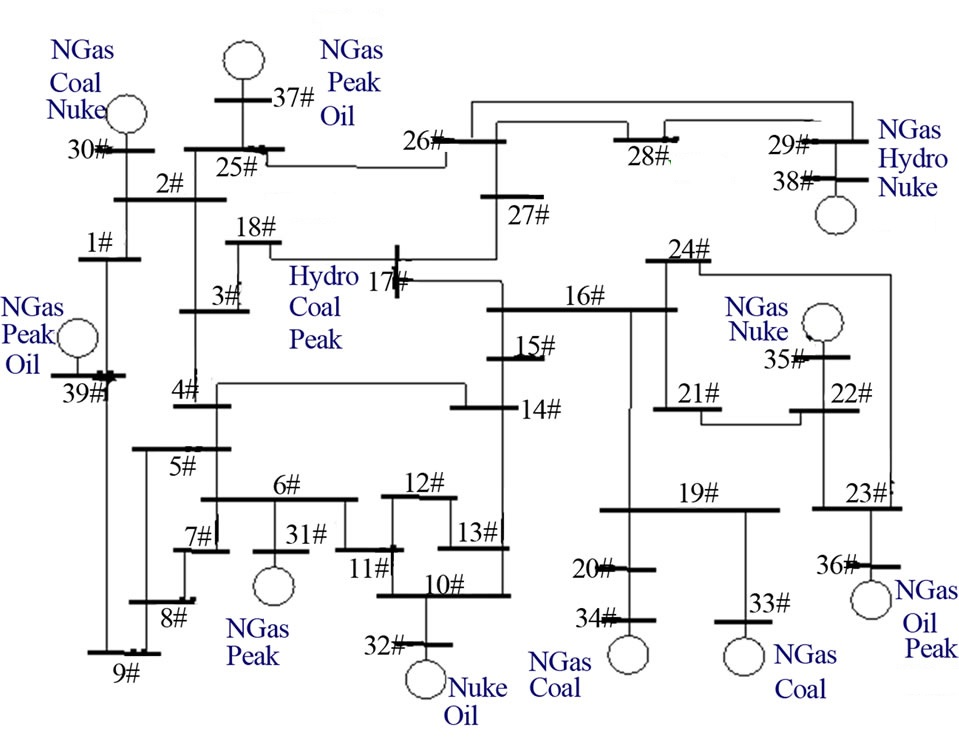
\includegraphics[width=1\columnwidth]{img/newEngland.jpg}
\caption{New England 39 bus test system}
\label{fig:newengland}
\end{figure}
%%%
}

\item{Datacenter model: \\
Based on the geographical mapping we aggregate all the datacenters in the New England ISO region into six datacenters, each datacenter for one state. In order to estimate the size of an "aggregated" datacenter in a certain state, we sue the follow equation:

\begin{equation}
L_i=\frac{n_i*9.8GW}{1278}
\end{equation}

\noindent where $L_i$ is the aggregated load of the $i$th state, $n_i$ is the number of datacenters reported in that state,  9.8GW is the upper bound of total electricity used by US datacenters in 2010, according to the report \cite{Koomey2011}, and 1278 is the number of datacenters in US collected and reported in \cite{DCmap}. However, according to \cite{Koomey2011}, for the summarized load of datacenters, there is an increase of 56\% from 2005-2010. Hence, we are assuming the increasing percentage from 2010-2014 is 56\%*0.8=45\%, and after adjustment we are using $L'_i=1.45L_i$ as the datacenter load for the target grid system.

The state wise aggregated datacenters are mapped to different buses according to their geographical locations, as seen from Table~\ref{tab:dc_setting}. Note that the load size given in the table represents the total load of datacenters in the entire state.

\begin{table}[ht]
\begin{center}
\caption{Background datacenter load and location settings}
\begin{tabular}{|l|l|p{30pt}|p{30pt}|p{30pt}|}
\hline
DC No. & State & Number of DCs & Estimated size(MW) & Mapped Bus No.\\
\hline
DC1 & Connecticut & 12 &133.43 & 6\\
DC2 & Maine & 3 &33.36 & 29 \\
DC3 & Vermont & 4 &44.48 & 25 \\
DC4 & Rhode Island & 3 &33.36 & 20\\
DC5 & New Hampshire & 4& 44.48 & 16\\
DC6 & Massachusetts & 27& 300.21 & 4 \\
\hline

\end{tabular}
   \vspace{.05in}
\label{tab:dc_setting}
\end{center}
\end{table}
}

\item{Wind farm model: \\
The wind farms connected to bus 18, 28, 36, 37 and 38 (Figure~\ref{fig:newengland}) are lumped models of several wind farms within a geographical region. The locations and capacity settings of the five wind farms are presented in Table~\ref{tab:wf_setting}. We assume that each farm can be represented by `$n$' identical wind turbines, where $n$= total farm rated capacity/individual wind turbine rating. This approximation does not change any of our results because we are interested in studying the global impact of wind farm powered datacenters on the electric grid. Also, since most of the wind turbines in this region are the GE 1.5MW machines, we consider the GE machine wind speed versus power characteristics \cite{lei2006modeling}. The wind speed versus turbine output characteristics is commonly referred to as the power curve (Figure~\ref{fig:windcurve}). From Figure~\ref{fig:windcurve} we can see that the cut-in wind speed, i.e., the wind speed at which the turbine starts producing power, is 5m/s and the cut-off wind speed is 25m/s, beyond this the turbine will be shut down for safety reasons. The wind turbine produces rated output (1.5MW) between wind speeds of 13-25m/s.
%%%
\begin{figure}[ht]
\centering
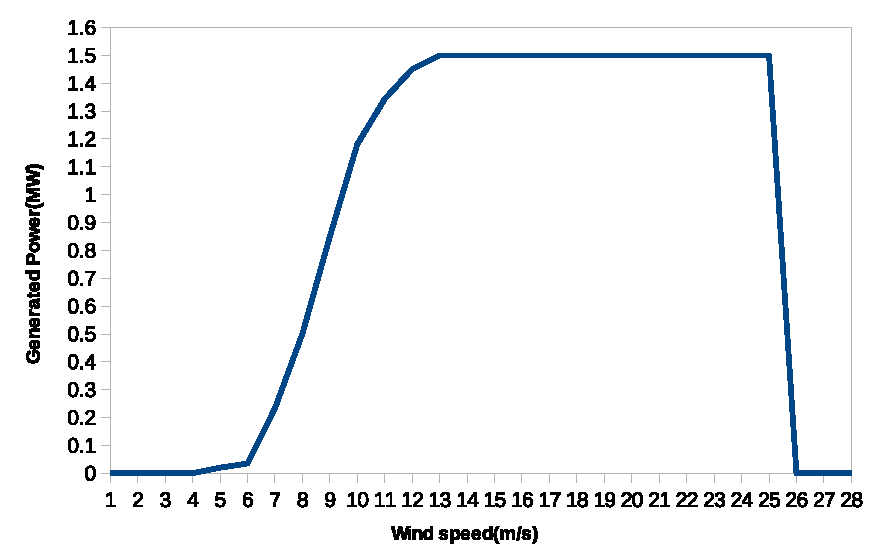
\includegraphics[width=1\columnwidth]{img/wind_curve.pdf}
\caption{Power curve of the GE 1.5MW wind turbine}
\label{fig:windcurve}
\end{figure}
%%%


\begin{table}[ht]
\begin{center}
\caption{Wind farm settings}
\begin{tabular}{|l|l|c|c|}
\hline
WF No. & Bus No. & State & Capacity(MW) \\
\hline
WF1 & 18& \xynote{?} & 100\\
WF2 & 28& \xynote{?} & 90 \\
WF3 & 36& Vermont & 90  \\
WF4 & 37& Maine & 90\\
WF5 & 30& Massachusetts(\xynote{?}) & 90\\
\hline

\end{tabular}
   \vspace{.05in}
\label{tab:wf_setting}
\end{center}
\end{table}
}
\end{itemize}
\subsection{Case study}
We have used the above described model and carried out the following case studies to assess the impact of datacenter location on the renewable power grid.
\begin{itemize}
\item{Case 1: Existing New England system}
\item{Case 2: New England system with one additional datacenter (co-located with a wind farm)}
\item{Case 3: New England system with one additional datacenter (located away from the wind farm)}
\end{itemize}
For assessing the impact, we use the three metrics described earlier (section \ref{sec:metrics}) and calculate the system losses, power flows through the transmission lines and the bus voltages.
The system losses, line flows and the bus voltages are calculated by solving the power flow or loadflow equations. The loadflow equations mathematically model the power balance (i.e., net load +losses = total generation in the electric grid). Within an electric grid the power can be easily measured at the loads and at generators. Also, some generators have the capability to regulate the voltage at a bus at a constant preset reference value. The power flow equations are used to calculate the bus voltages (magnitude and angle), for a given network and a set of load and generation powers. The loadflow equation for a generic $n$ bus network with $k$ branches is given below.
\begin{equation}
P_{i} = \Sigma_{j=1}^{n}(|Y_{ij}||V_{i}||V_{j}|cos(\theta_{ij}+\delta_{j}-\delta_{i})
\end{equation}
\begin{equation}
Q_{i} = -\Sigma_{j=1}^{n}(|Y_{ij}||V_{i}||V_{j}|sin(\theta_{ij}+\delta_{j}-\delta_{i})
\end{equation}
where $P_{i}$ and $Q_{i}$ are real and reactive powers at the $i^{th}$ bus; $|V_{i}| \angle \delta_{i}$ is the voltage magnitude and angle at the the $i^{th}$ bus; $|Y_{ij}| \angle \theta_{ij}$ is the admittance of the branch between $i^{th}$ and $j^{th}$ bus.
For a given power $P_{i}$ and $Q_{i}$ at the $i^{th}$ load bus, the above powerflow equations are used to solve for the voltage magnitude and angle at the $i^{th}$ bus. Since the above equations, i.e., real and reactive powers are non-linear function of voltage they are solved iteratively using Newton Raphson method. Once the bus voltages are calculated the line flows and system losses are computed.
\subsection{Results and discussion}
%I need only the following results for each case (Case1, Case2 and Case 3):
%1. a table containing system losses for each case (total loss its only one number for each case)
%2. any line capacity violations (line number)
%3. voltage violations if any (bus number)
%%%

Here, we show the simulation results of the three cases and investigate the situation of line overloading, voltage variation and the value of system losses under the condition of different placement choices. 

First, we conduct experiments using peak system load (6885MW in total) and gain an insight of the impact of datacenter placement on line overloading situations. Wind speed setting here is LOW (4-6m/s), which means the power generated by the wind farm is nearly zero (less than 2.3\% of the rated capacity). Evaluation results are illustrated in Table \ref{tab:results-linevio}, which shows that there is one overloaded branch from bus 4 to bus 5 in Case 2. This highlights that different placement choice of the additional datacenter can make some particular lines overloaded. During our experiments, although there are only a few cases where lines are overloaded, annually the number of times and how long these over-loads could occur depends on the frequency and duration of occurrence of a particular wind speed and load condition. If it is too frequent or more persistent then the over-loads could be a serious problem and might require building new transmission lines. According to \cite{interconnection2010survey}, the estimated cost of building new transmission lines of 345kV voltage level is about \$2.5 Million/mile, which is very expensive with total costs in the billions of dollars. Hence, it's important to choose the right place for datacenters in order to mitigate line over-loading occurrences.


\begin{table}[ht]
\begin{center}
\caption{Results of overloaded lines}
\begin{tabular}{|c|c|c|}
\hline
Case No. & \# of overloaded lines & List of overloaded lines \\
\hline
1 & 0 & None\\
2 & 1 &  bus 4 - bus 5 \\
3 & 0 & None \\

\hline

\end{tabular}
   \vspace{.05in}
\label{tab:results-linevio}
\end{center}
\end{table}

Then, we investigate cases illustrating voltage variation of the electric grid, as shown in Table \ref{tab:results-volvio}. Here, the wind speed setting is MEDIUM (8-10m/s), which means the generated power of the wind turbine will be 33.3\%-78.7\% of its rated capacity. For Case 2 the datacenter is located at bus 38 (co-located with wind farm 5), and for Case 3 the datacenter is located at bus 25 (away from wind farms). The acceptable voltage range of a bus is set to [0.95p.u.,1.05p.u.]. It can be observed under this condition, there is already voltage deviation happening on one bus of the original New England system. When we choose a place for the datacenter co-locating with a wind farm as Case 2, the number of buses with voltage deviation will increase to four. If we don't restrict to co-located datacenter placement, we can find other possible choices (e.g. Case 3) to eliminate the unacceptable voltage deviation from nominal values. This result highlights that by carefully choosing the place for the datacenter might mitigate large voltage variations of the electric grid.

\begin{table}[ht]
\begin{center}
\caption{Results of voltage variations}
\begin{tabular}{|c|p{1in}|p{1in}|}
\hline
Case No. & \# of buses with voltage deviation & List of buses with voltage deviation  \\
\hline
1 & 1 & bus25\\
\hline
2 & 4 & \tabincell{c}{bus25\\bus26\\bus28\\bus29}\\
\hline
3 & 0 & None \\

\hline

\end{tabular}
   \vspace{.05in}
\label{tab:results-volvio}
\end{center}
\end{table}

At last, the total system losses are compared over the three cases under the condition of three wind speed settings, as shown in Figure~\ref{fig:loss-cases}. Here, the background load of the electric grid is set to normal (6254MW in total,summarized over all the buses). Three categories of wind speed settings are: LOW, MEDIUM, and HIGH. The setting HIGH means the wind speed is larger than 11m/s, and the output power of the wind turbine is nearly reaching its rated capacity. For example, a 100MW wind farm is generating at least 89.6MW power under this setting. The size of the additional datacenter in Case 2\&3 is set to 200MW. Specifically, for Case 2 the datacenter is located at bus 18 (co-located with wind farm 1) and for Case 3 the datacenter is located at bus 10 (away from all wind farms).

\begin{figure}[ht]
\centering
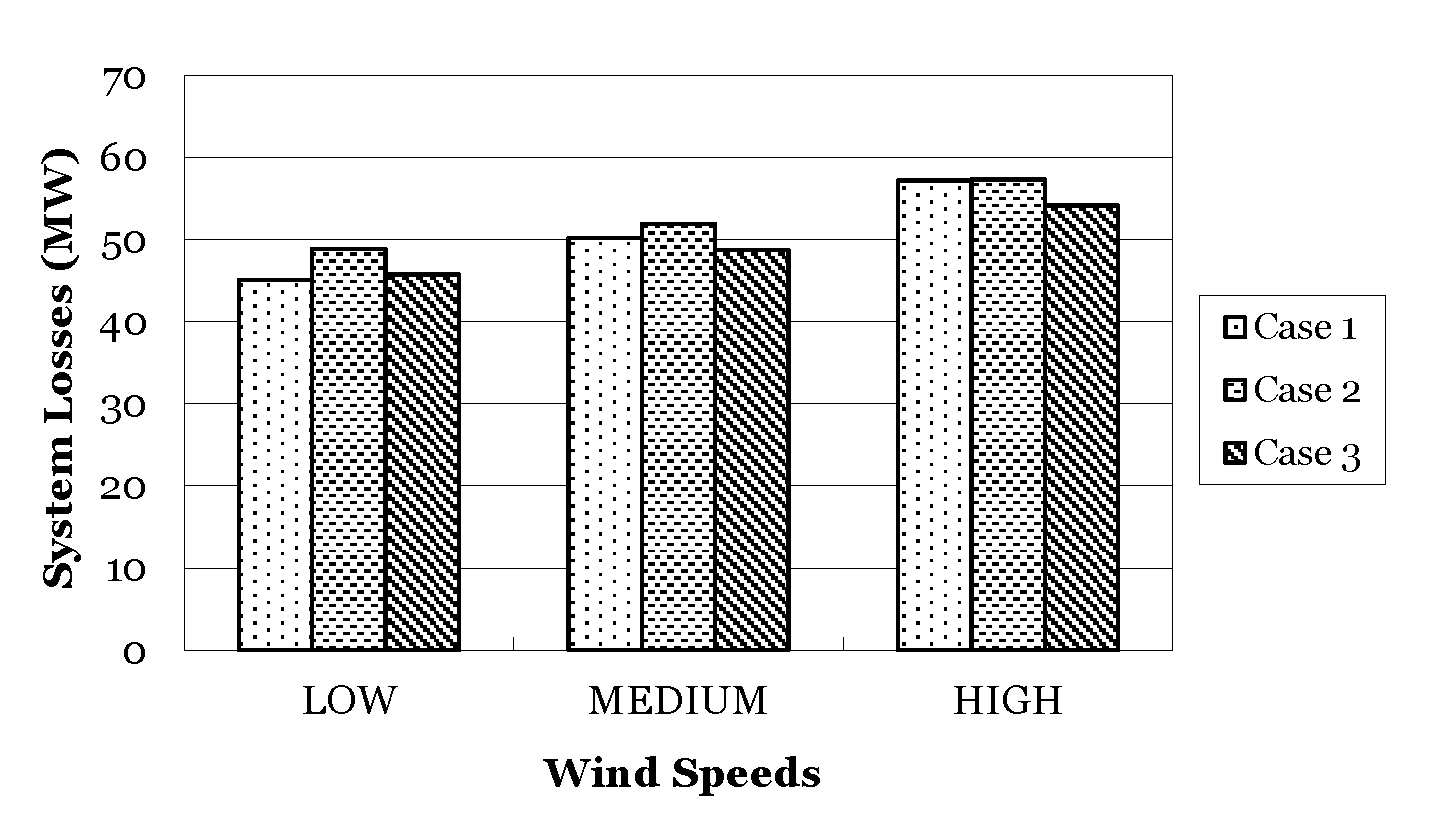
\includegraphics[width=1\columnwidth]{img/loss3cases.pdf}
\caption{Results of system losses}
\label{fig:loss-cases}
\end{figure}

By comparing the values of system losses from Figure~\ref{fig:loss-cases}, it can be observed that the co-location case (Case 2) could lead to more losses than Case 1 and Case 3. Take MEDIUM setting for example, the system losses of Case 3 is about 6\% less than Case 2, which illustrates system loss can be reduced by placing the datacenter correctly and co-location is not necessarily the best choice.


Note that even though we have provided one set of results for a particular set of condition, we have simulated different wind speed and load conditions. We found that in general the system loss magnitude could change. However, in most cases we saw that co-location is not the optimal choice for minimum system loss. In Section \ref{sec:framework} we will describe a method for determining the datacenter location that will correspond to minimal system loss annually and will cover all the wind speed and system load conditions.


\section{Cost-based Placement}
\label{sec:framework}

As shown in the last section, the placement of new datacenters and wind farms can have significant impact on a grid transmission system.  As previously shown in~\cite{berral2014building,Goiri11place}, the placement of datacenters can also significantly impact their costs.  Thus, in this section, we develop an optimization framework for placing new renewable powered datacenters that unifies the impact of location on the costs of datacenters and loss in the transmission grid.  For simplicity, we assume that one datacenter and one wind farm are being placed in the system simultaneously.  Our framework can be easily extended to account for the simultaneous placement of multiple datacenters and multiple wind farms; of course, solving the optimization problem can become much more challenging for such cases.  Our optimization seek to find locations for the datacenter and wind farm that lead to the lowest total cost for construction and operation.  The overall framework is based on computing the cost throughout a year, using amortized capital costs and operational costs for the datacenter and operational revenue of the wind farm, along with system loss in the transmission network.

% By grid-aware placement, we attempt to efficiently select a set of locations for one or more datacenters to support a given amount of computational power, as well as one or more green power plants (e.g. solar, wind or others) to provide a given power capacity. The main goal is to minimize the overall cost for datacenters, green power plants and also the grid network operation. The next subsections defines some important parameters in the selection procedure. Then, the cost model and the entire optimization problem will be formulated and described.

\begin{table}[t]
\caption{Framework parameters.  $l$ is a location, and $t$ is a time period.}
\begin{center}
\begin{tabular}{|l|p{1.9in}|r|}
\hline
\textbf{Symbol} & \textbf{Meaning} & \textbf{Unit}\\
\hline
$dcCapacity$ & desired power capacity for computing in DC & kW \\
$wfCapacity$ & desired power production capacity of wind farm & kW \\
\hline \hline
$pLand(l)$ & land price at $l$ & \$/m$^2$ \\
\hline \hline
$PUE(l,t)$ & PUE at $l$ during $t$ & \\
$maxPUE(l)$ & maximum PUE at $l$ & \\
$dcArea$ & land needed per kW of DC compute capacity &  m$^2$/kW \\
$cLinePow(l)$ & cost to layout power line from $l$ to the closest power plant & \$ \\
$cLineNet(l)$ & cost to layout optical fiber from $l$ to closest network backbone & \$ \\
$pBuildDC(c)$ & per kW price of building a datacenter with $c$ power capacity & \$/kW \\
$serverPow$ & server peak power demand & kW/serv \\
$switchPow$ & switch peak power demand & kW/switch \\
$servsSwitch$ & number of servers per switch & servs/switch \\
$pServer$ & price of a server &  \$/serv \\
$pSwitch$ & price of a network switch & \$/switch \\
$pNBWServ$ & cost of external network bandwidth per server & \$/serv-month\\
$pEnergy(l)$ & grid electricity price at $l$ & \$/kWh \\
$powNeed(t)$ & avg computing power demand of DC during $t$ &  kW \\
\hline \hline
$\beta(l,t)$ & avg generation efficiency of wind energy at $l$ during $t$ &  \%  \\
$wfArea$ & land needed per kW wind power & \$/m$^2$ \\
$pBuildWF$ & per kW price of building a wind power plant & \$/kW \\
%$avgEff(l)$ & avg generation efficiency of wind energy at $l$ & \% \\
$revEnergy(l)$ & revenue for selling wind energy to grid at $l$ & \$/kWh \\
\hline \hline
$transLoss(t)$  & avg system transmission loss in grid during $t$ & kW \\
%$disLoss(t)$ & the losses for distributing power to datacenter during time epoch $t$ & kW \\
$pTransLoss$ & the price for system transmission losses per kWh & \$/kWh \\
%$numLineVio(t)$  & the number of line capacity violation during time epoch $t$   &  \#  \\
%$numVolVio(t)$  & the number of voltage level violation during time epoch $t$  &  \#  \\
% $V_i$ & the voltage level of the $i$th bus & p.u. \\
% $V^{min}_i$ & the minimum accepted voltage of the $i$th bus &p.u.\\
% $V^{max}_i$ & the maximum accepted voltage of the $i$th bus & p.u. \\
% $P_k$ & the current line flow on the $k$th branch & MW \\
% $P^{max}_k$ & the maximum allowed line flow of the $k$th branch & MW \\
\hline
\end{tabular}
\label{tab:par_setting}
\end{center}
\vspace{-0.1in}
\end{table}

\subsection{Optimization Framework}

Table \ref{tab:par_setting} lists the set of parameters in our framework.  Using these parameters, we define the optimization problem shown in Figure~\ref{fig:optimization}.  The objective of this optimization problem is to minimize the total cost ($totalCost$) of building and operating a datacenter of a given size ($dcCapacity$) and a wind farm of a given size ($wfCapacity$). %\xynote{In the program, wind farm size is not given but calculated based on the datacenter size and other location-dependent parameters.}
The datacenter and wind farm can each be placed at any location within a set of given locations.  The total cost has three components, the cost of the datacenter ($dcCost$), the cost of the wind farm ($wfCost$), and the cost of losses in the transmission system ($transCost$).

\begin{figure*}
% Minimize $totalCost$ subject to
% \begin{eqnarray}
% V^{min}_i  \leq  V_i \leq V^{max}_i\\
% P_k \leq P^{max}_k
% \end{eqnarray}
% where
{\small
\begin{eqnarray}
 	totalCost & = & dcCost + wfCost + transCost \\
	dcCost & = & dcCAPEX + dcOPEX \\
        dcCAPEX & = & dcLandCost + dcBuildCost + dcITCost \\
        dcOPEX & = & dcNetCost + dcEnergyCost \\
        dcLandCost & = & pLand(d) \cdot dcArea \cdot dcCapacity \\
        dcBuildCost & = & dcTotalPow \cdot pBuildDC(dcTotalPow) +
            cLinePow(d) + cLineNet(d) \\
        dcTotalPow & = & dcCapacity \cdot maxPUE(d) \\
        dcITCost & = & nServers \cdot pServer + nSwitches \cdot
            pSwitch \\
        nServers & = & dcCapacity / (serverPow + switchPow / servsSwitch)\\
        nSwitches & = & nServers / servsSwitch\\
        dcNetCost & = & nServers \cdot pNBWServ \\
        dcEnergyCost & = & \sum_{t \in T} {|t| \cdot powNeed(t) \cdot PUE(d,t) \cdot pEnergy(d) } \\
 	wfCost & = & wfCAPEX - wfRev  \\
        wfCAPEX & = & wfLandCost + wfBuildCost \\
        wfLandCost & = & pLand(w) \cdot wfArea \cdot wfCapacity \\
        wfBuildCost & = & pBuildWF \cdot wfCapicity + cLinePow(w) \\
        wfRev & = & revEnergy(w) \cdot  \sum_{t \in T}{ |t| \cdot
            \beta(w,t) \cdot wfCapicity } \\
        transCost & = & pTransLoss \cdot \sum_{t \in T}{ |t| \cdot transLoss(t)} % + disLoss(t))}\\
\end{eqnarray}
}
\caption{Optimization framework with objective of minimizing $totalCost$.  The datacenter is placed at location $d$ and the windfarm is placed at location $w$.  The objective is to minimize $totalCost$ for a given time period $T$ (divided into epochs denoted by $t$) and a set of possible locations for $d$ and $w$.  $|t|$ denotes the length of epoch $t$.}
\label{fig:optimization}
\vspace{-0.2in}
\end{figure*}


\subsubsection{Datacenter} The cost of the datacenter can be broken down into capital ($dcCAPEX$) and operational ($dcOPEX$) components.  The capital costs are those investments made upfront and depreciated over the lifetime of the datacenter.  These costs include the cost for buying land ($dcLandCost$), building the datacenter ($dcBuildCost$), and buying IT equipment ($dcITCost$).  The cost of building the datacenter include datacenter construction cost as well as the costs of laying power and network lines to the datacenter.  IT equipment includes servers and switches.  Land price varies according to location ($pLand(d)$ for location $d$), whereas the other prices do not to a first approximation.  Of course, the total cost of laying the power ($cLinePow(d)$) and network ($cLineNet(d)$) lines depends on location, as the distances to the closest power plant and network backbone are location-dependent.  The datacenter construction cost is typically estimated as a function of the maximum power to be consumed by the datacenter.  This maximum power is that required by the maximum number of servers and network switches when running at 100\% utilization times the maximum expected PUE of the datacenter.  The PUE is computed by dividing the overall power consumption by the power consumption of the computational equipment.  The PUE is higher when temperature and/or humidity are high, since cooling consumes more energy under those conditions.

The operational costs are those incurred during the operation of the datacenter over the time period $T$, and include costs for external network bandwidth use ($dcNetCost$) and the grid electricity ($dcEnergyCost$) required to run the datacenter.
%(There is also a cost for water, which is currently not considered by can be easily added.)
The electricity cost is computed based on the IT equipment's power demand over time ($powNeed(t)$), the PUE, and the electricity price.  Both the electricity price and the PUE vary with location.

% Finally, lower taxes and one-time incentives are another important component of the cost of a datacenter.  For example, some states in the US lower taxes on datacenters, as they generate employment and wealth around them.  This component depends on the nature of the savings and applies to each cost in a different way.  Although we do not consider this component further, it is easy to add it to our framework.

\subsubsection{Wind farm}  The cost of the wind farm is modeled as the capital cost ($wfCAPEX$) minus the revenue earned by selling the wind energy to the grid ($wfRev$).  We assume that the operational cost of operating the wind farm is low, and so do not consider it here; of course, this cost can be easily added to the framework.  The capital costs include the cost for buying land ($wfLandCost$) and building the wind farm ($wfBuildCost$), which in turn includes the construction cost and the cost of laying the power line from the wind farm to the closest power plant.  The construction cost is assumed to be a linear function of the desired power generation capacity.  Note that if the datacenter and wind farm are co-located, then the cost for laying power lines is incurred only once.

The revenue earned by the wind farm is computed over the time period $T$, where the energy generated within any time epoch $t$ in $T$ at location $w$ depends on the efficiency of the wind turbines and the wind speed.  The efficiency of today's wind turbine is close to 50\%.  We capture the efficiency and impact of wind speed in epoch $t$ using the parameter $\beta(w,t)$, which gives the fraction of the wind farm's maximum capacity actually produced during $t$.

\subsubsection{Transmission system} As discussed above, adding a datacenter and wind farm to an existing transmission system will alter the power flow of the network, thus affecting the system transmission loss.  We model this loss across the entire time period $T$, and assume that each unit of loss has a corresponding cost.  For each potential placement of the datacenter and wind farm, we compute the system loss for each time epoch $t$ using the power flow and loadflow equations described in Section~\ref{sec:quantify}.

% On the other hand, during the transmission process the line capacity might be violated if the power flow exceeds the limit. We use $numLineVio(t)$ and $numVolVio(t)$ to denote the number of line capacity violations and voltage violations during power transmission. The grid operator will try to avoid such violations when operating the power grid system.


\subsubsection{Constraints}

The major constraints that must be observed when optimizing is that there must not be any voltage and transmission line capacity violations.

\subsection{Solving the Optimization Problem}

Currently, we perform a complete search over all possible placement of the datacenter and wind farm to find the best solution to the optimization problem.  This approach works well for the scale that we are studying (e.g., the New England system).  However, as the system scale to much larger sizes, a more scalable approach would eventually be needed.  We leave this for future work.  (Note that the New England system that we study already covers a large area -- most of the North Eastern region of the U.S. and some parts of Canada -- so that it may not be necessary to study much larger systems.)

% datacenters and renewable power plant, as well as the capacity provisioned at each location for datacenters or green power plants (if any).

% The overall cost should be optimized under the constraints, which are listed in Figure~\ref{fig:constraints}. Equation 21-23 show the constraints of the provisioned capacity for datacenters.

% Equation 24 means that the provisioned capacity for renewable energy plants are determined by the total power demand from the datacenters. This constraint is added indicating that the power generation and consumption added to the grid should be balanced from the perspective of the grid system.

% Furthermore, Equation 26
% is a strict limitation for keeping the grid out of any violations at any given time $t$, since we assume the grid reliability is crucial and must be guaranteed.

% \begin{figure*} [ht]
% \begin{small}
% \centering
% \begin{eqnarray}
% \forall_{l \in \mathcal{L}}, capDC(l) \leq DC(l) \cdot CapacityDC
% &\Rightarrow& \text{capacity of datacenter at $l$ should be zero when $DC(l)$ is 0} \\
% \sum_{l\in \mathcal{L}}{DC(l)\cdot capDC(l)} = CapacityDC
% &\Rightarrow& \text{total capacity of built datacenters should meet the requirement} \\
% \forall_{t \in T}, demand(l,t) \leq capDC(l)
% &\Rightarrow& \text{power demand of the datacenter should not exceed its capacity} \\
% %\forall_{l \in \mathcal{L},r\in \mathcal{R}}, capRE(l,r) \leq RE(l,r) \cdot CapacityRE  & \Rightarrow &
% %\text{capacity of type $r$ plant at $l$ should be zero if $RE(l,r)$ is 0} \\
% %\sum_{l \in \mathcal{L},r \in \mathcal{R}}{RE(l,r) \cdot capRE(l,r)} = CapacityRE & \Rightarrow &
% %\text{total capacity of power plant should meet the requirement}\\
% \begin{split}
% \sum_{l \in \mathcal{L},r \in \mathcal{R}}{ RE(l,r) \cdot capRE(l,r) \cdot avg\textit{Eff}(l,r) } = \\
% \sum_{t \in T, l\in \mathcal{L}}{DC(l) \cdot demand(l,t)\cdot PUE(l,t)}
% \end{split}
% &\Rightarrow &\text{the generated green energy should be balanced with consumption} \\
% \forall_{t \in T}, 0 \leq \textit{eff}RE(r,l,t) < 1
% &\Rightarrow&  \text{efficiency of power plant should be between $[0,1)$} \\
% \forall_{t \in T}, numLineVio(t)=0, numVolVio(t)=0
% &\Rightarrow& \text{No violations in each time epoch}
% \end{eqnarray}
% \end{small}
% \caption{Optimization constraints.}
% \label{fig:constraints}
% \end{figure*}

%%% Local Variables:
%%% mode: latex
%%% TeX-master: "paper"
%%% End:

\subsection{Case Study}
\label{sec:eval}

We now demonstrate the application of our optimization framework in a case study.  Specifically, we use it to study the placement of a 100MW datacenter and wind farm in the New England transmission network.  Instead of specifying a desired capacity for the wind farm, we assume that we want sufficient wind energy to completely offset the energy consumption of the datacenter (making the size of the wind farm dependent on the weather pattern at its placement location).  This scenario corresponds to when a company wants to build a new datacenter, and a corresponding wind farm to offset the energy use of the datacenter.

\subsubsection{Instantiating the framework parameters}

The production of wind power and datacenter cooling both depend on weather conditions.  Thus, we obtained Typical Meteorological Year (TMY) information for 56 locations in the U.S. New England area as shown in Figure~\ref{fig:NE_locs}.  A TMY is a 1-year dataset of hourly weather values selected to include a representative range of weather phenomena for a location, while still giving annual averages that are consistent with the long-term averages for the location.  The TMY data is obtained from US Department of Energy.\footnote{\url{http://apps1.eere.energy.gov/buildings/energyplus/weatherdata about.cfm}} We use the TMY wind speeds and air pressures, conversion losses, and specifications for the 1.5MW Series wind turbine from General Electric Company \cite{GE15MW} to compute $\beta(l,t)$ at each location $l$ during time epoch $t$.

\begin{figure}[ht]
\centering
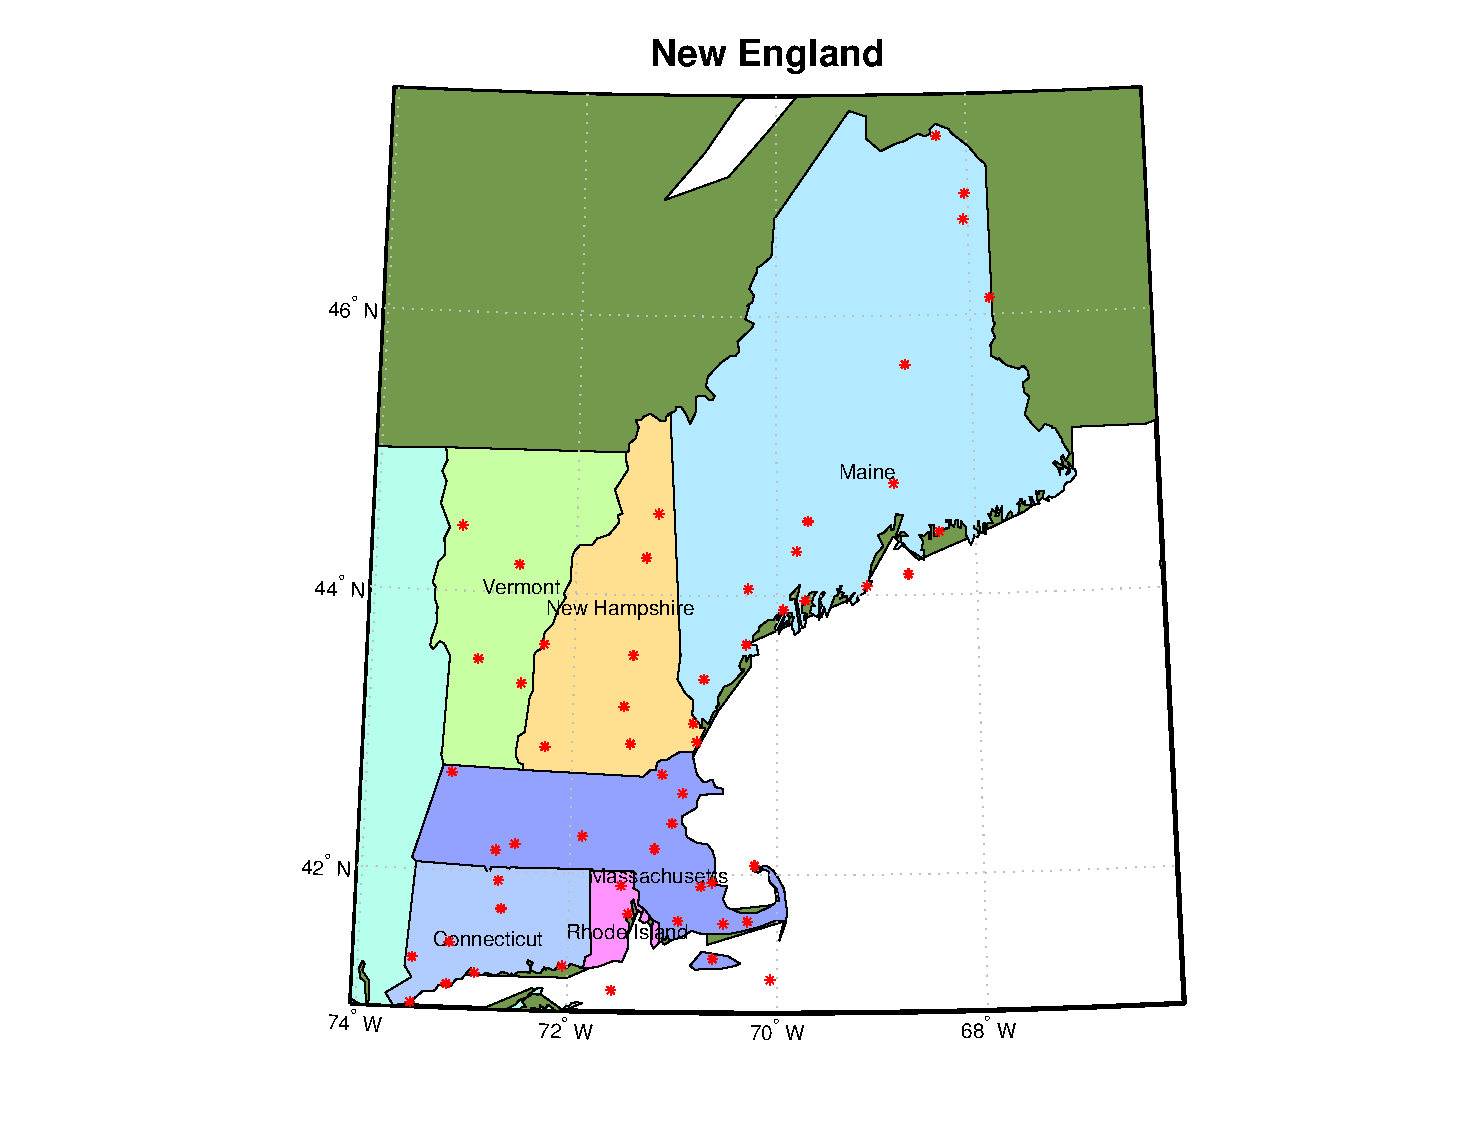
\includegraphics[width=1\columnwidth]{img/NE_map}
\caption{Candidate locations in New England}
\label{fig:NE_locs}
\end{figure}

We adopt the values and approaches for computing PUE, datacenter construction costs, wind farm construction costs, land costs, transmission lines and network connection costs, and grid energy costs from \cite{berral2014building}.  Table \ref{tab:loc-dependent-pars} shows part of the location-dependent parameters for five typical locations used in our experiments, and Table \ref{tab:constant-pars} shows the values of the location-independent parameters. \thunote{I think we need a summary table here to give information.}

\begin{table}[ht]
\begin{center}
\caption{Location-dependent parameter settings for five typical locations.}
\begin{tabular}{|l|p{22pt}|p{28pt}|p{20pt}|p{27pt}|p{27pt}|}
\hline
\textbf{Locations}& Burlinton, NH&Springfield Hartnes, VT&Nash Island, CO&Marthas Vineyard, RI & Mount Washington, NH
\\
\hline
$pLand$ (\$/m$^2$)&946.9&946.9&946.9&680.21&946.9  \\
$maxPUE$&1.0650&1.0639&1.0698&1.0639&1.0601 \\
$cLinePow$ (M\$)&64.5&77.2&16.6	&86.6&107.1 \\
$cLineNet$ (M\$)&13.5&16.7&16.9&17.7&21.3 \\
$pEnergy$ (\$/kWh)&0.0941&0.0941&0.1281&	0.1281&	0.1257 \\
Average $\beta$ (\%) &11.7&2.7&	40&	15.9&56.8 \\
\hline
\end{tabular}
\label{tab:loc-dependent-pars}
\end{center}
\end{table}

\begin{table}[ht]
\begin{center}
\caption{Values of location-independent parameters.}
\begin{tabular}{|l|c|}
\hline
\textbf{Parameter}& \textbf{Value} \\
\hline
$dcArea$ (m$^2$/kW)&	0.557 \\
$\textit{pBuildDC}$ (\$/kW)	&12000 \\
$serverPow$ (kW/serv)	&0.275 \\
$switchPow$ (kW/switch)	&0.48 \\
$servsSwitch$ (servs/switch)&	32 \\
$pServer$ (\$/serv)	&2000 \\
$pSwitch$ (\$/switch) & 20000 \\
$\textit{pNBWServ}$ (\$/serv-month)&	1 \\
$wfArea$ (\$/m$^2$)&	18.21 \\
$\textit{pBuildWF}$ (\$/kW)&	2.1 \\

\hline
\end{tabular}
\label{tab:constant-pars}
\end{center}
\end{table}



\thunote{Xiaoying, what is the assumed load?  What about the datacenter load ($powNeed$)}
For each time epoch $t$, we compute the wind energy being generated by all the wind farms (existing ones and the new one being placed) using $\beta(l,t)$.  We then compute the system loss for the time epoch for the placement of the new datacenter and wind farm at locations $d$ and $w$, respectively, using the simulation approach described in Section~\ref{sec:quantify}.  For each possible pair of ($l$, $w$), we sum the transmission loss over the entire year.

Finally, for the cost of system transmission loss, we set $pTransLoss$ to the maximum electricity price in the whole area.  \thunote{Xiaoying, Divya gave us some values that we can use here.  Did we use these new values, or are we still using the maximum electricity price?}

\subsubsection{Placement approach}

To see the impact of considering transmission loss, as well as the simultaneous placement of datacenter and wind farm, we compare results for five different placement approaches:

\begin{itemize}

\item \textbf{DC\_WF\_OPT:} This strategy individually looks for the best location to put the datacenter and the wind farm; i.e., it solves the optimization problem for the datacenter without considering the new wind farm, and then solves the optimization problem again for the wind farm without considering the new datacenter.  This strategy also ignore transmission loss.

\item \textbf{DC+G\_WF+G:} This strategy is the same as DC\_WF\_OPT except that transmission loss is considered when solving the optimization problem.

\item \textbf{Min\_Loss:} This strategy finds locations for the datacenter and wind farm that minimizes the cost of transmission loss.

\item \textbf{Co-location:} This strategy assumes that the datacenter and wind farm
should be co-located, and so finds a single location for both that minimizes the overall cost.

\item \textbf{Jointly:} This strategy considers the simultaneous placement of the datacenter and wind farm, and uses all of the costs and revenues in the optimization framework.

\end{itemize}

\subsubsection{Results}
Figure \ref{fig:cost1dc1wf} shows the results of the total cost by using five different strategies when seeking the best locations when we are building a 100MW datacenter and a wind farm which can supply green energy for it.

From the figure, we can see that by considering grid costs, the total cost will be further saved compared to best choices for the datacenter and the wind farm separately. Also, $Min\_Loss$ can achieve minimal losses of all possible choices, but the total cost is large mainly because it selects an expensive place for purchasing land for the wind farm. The best choice of co-location options is also nearly 7\% higher than the $Jointly$ choice, and it's easy to understand since the best location for datacenter is not necessarily the best for wind farm and vice versa.

We calculate all of the combinations for wind farm and datacenter locations and use the average total cost of these combinations (which is \$667.1M per year) as the baseline for comparison. Then, the locations found and the corresponding cost savings of the five strategies are listed in Table \ref{tab:costsaving}.

\begin{figure}[ht]
\centering
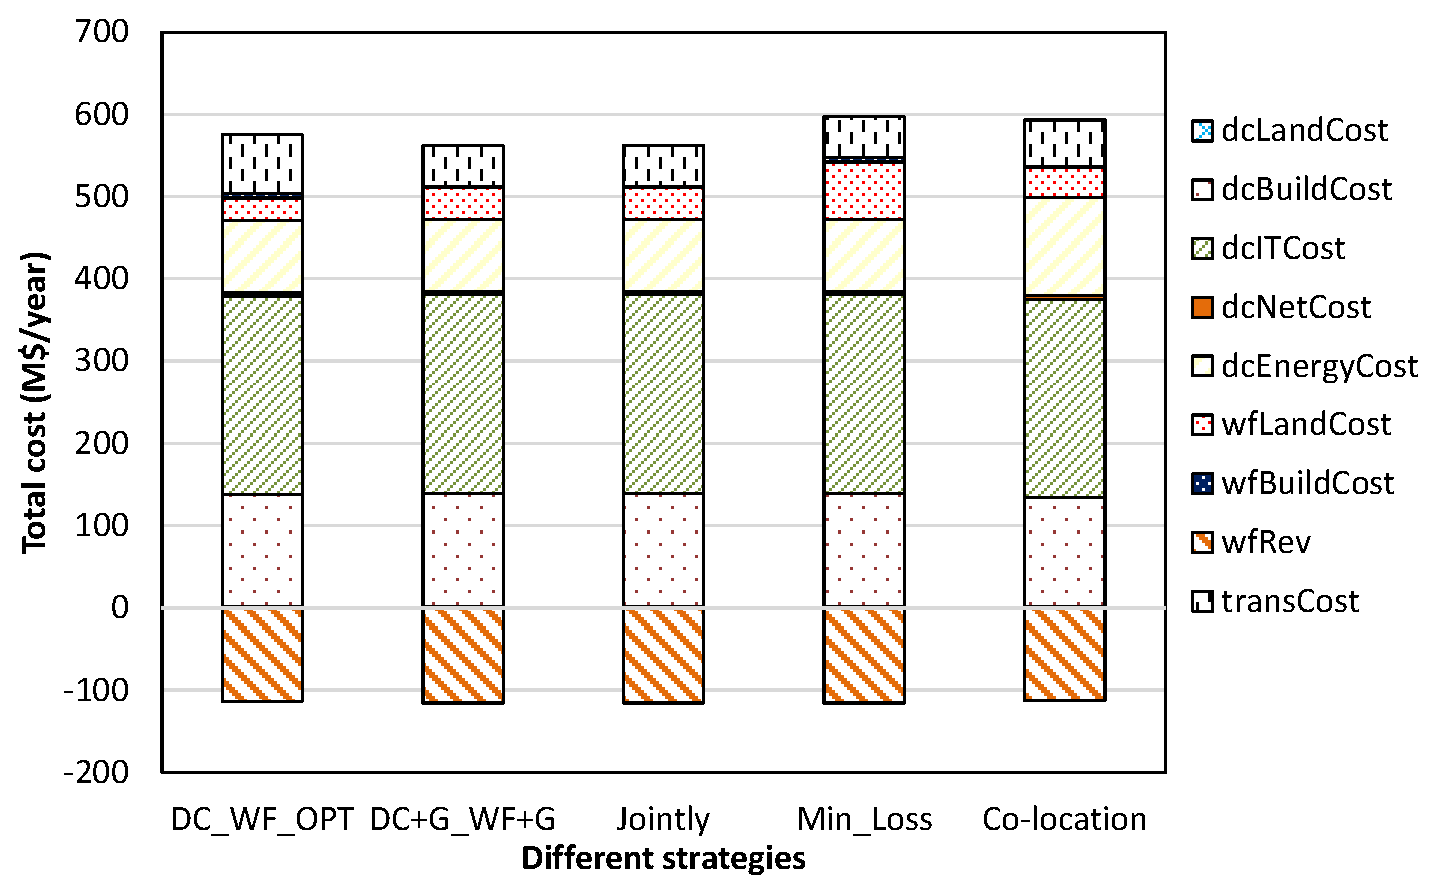
\includegraphics[width=1\columnwidth]{img/cost-one-dc-one-wf}
\caption{Costs of building one datacenter (100MW) with one wind farm}
\label{fig:cost1dc1wf}
\end{figure}

\begin{table}[ht]
\begin{center}
\caption{Detailed results of cost savings by different strategies.}
\begin{tabular}{|l|p{50pt}|p{50pt}|p{30pt}|p{20pt}|}
\hline
\textbf{Strategy}& \textbf{Datacenter location} &\textbf{Wind farm location} &\textbf{Total cost (M\$/year)} &\textbf{Cost saving (\%)} \\
\hline
\textbf{DC\_WF\_OPT} &  Burlington,NH  & Mount Washington, NH &465.6& 30.2 \\
\textbf{DC+G\_WF+G} &Springfield Hartnes, VT  & Nash Island, CO&450.3& 32.5\\
\textbf{Jointly} &Springfield Hartnes, VT&  Nash Island, CO & 450.3 & 32.5\\
\textbf{Min\_Loss} &Springfield Hartnes, VT & Marthas Vineyard, RI & 485.6& 27.2 \\
\textbf{Co-location}& Nash Island, CO &Nash Island, CO&480.7 & 27.9  \\
\hline
\end{tabular}
\label{tab:costsaving}
\end{center}
\end{table}

%%% Local Variables:
%%% mode: latex
%%% TeX-master: "paper"
%%% End:

\section{Related Work}
\label{sec:related}

As already mentioned, a number of previous efforts have studied the
placement of new datacenters.  Alger \cite{Dalger05} explained how to
choose an optimal location for a datacenter by considering hazards,
accessibility, and scalability factors.  Stansberr \cite{Stansberr06}
ranked some cities by estimating the annual operation costs of a
datacenter.  Oley \cite{Boley09} considered looking for a proper
location for a datacenter by investigating the
power rates of different states.  Goiri $\textit{et al.}$
\cite{Goiri11place} focused on intelligently finding the best places
for building multiple datacenters to form a network for interactive
Internet services.  Berral $\textit{et al.}$ \cite{berral2014building}
considered selecting sites for datacenters and on-site power plants
that support ``follow-the-renewables'' cloud services.  Gao $\textit{et al.}$
\cite{gao2013answer} studied how to site datacenters near existing
wind farms, and distributing load using a greedy online algorithm.
None of these works have considered the impact of placing new
datacenters on the transmission grid. 

A previous work that has considered the interaction of datacenters and
the grid is~\cite{liu2014pricing}.  In this work, Liu $\textit{et
  al.}$ show that adding renewable power plants (solar in their study)
can lead to voltage violations within a grid distribution system.
They also show that datacenters can help avoid such voltage
violations by dynamically adjusting their power demand based on
signals from the grid.  A number of research efforts have also studied
how datacenters can participate in demand response programs and
ancillary services to help ease the management of the
grid~\cite{Aikema12,AdamWierman2014}.  A key difference between these
works and ours is the assumption of datacenters being able to
dynamically adjust their power demands in response to grid signals.
In addition, they did not actually consider the placement of
datacenters, nor did they consider transmission system losses.

Mohsenian $\textit{et al.}$ in \cite{Mohsenian-Rad10grid} proposed a
request distribution policy among datacenters to ensure power load
balancing. They tried to minimize the maximum power on any
transmission line by distributing the computing requests to suitable
datacenters. Their work assumes that a fairly large number of
datacenters (e.g., 6) are connected to the same power distribution
network.  Further, they did not consider the impact of transmission system losses on the placement of datacenters.

% Larumbe $\textit{et al.}$ \cite{larumbe2012optimal} presented a mathematical problem aiming at solving the location and routing of cloud service components.
% Unlike our work, they didn't put insights the possible impact of datacenters and distributed energy generations on the utility grid system.
% A very close paper to our work is \cite{liu2014pricing} which considered a realistic distribution system and discussed how it impacts the voltage in the distribution system, while we are focusing on the transmission system of the grid.



%%% Local Variables:
%%% mode: latex
%%% TeX-master: "paper"
%%% End:

\section{Conclusion}
\label{sec:conclusion}

In this paper, we proposed that new renewable powered datacenters should be placed intelligently while considering their impact on the electricity transmission system (along with other datacenter capital and operation costs).  Specifically, we studied the potential impact of new datacenters on the New England ISO transmission system.  Using simulation, we show that different placements of a new datacenter and its offsetting wind farm can lead to increased overloading of transmission lines, grid voltage variations outside the acceptable range, and transmission system losses.  Thus, strategic placement of new renewable powered datacenters can be beneficial for both grid operators and datacenters owners.  We developed an optimization framework for the placement of a new datacenter and offsetting wind farm\red{, which can be easily extended to simultaneous placement of multiple data centers and multiple wind farms.
Our algorithm shows the importance of considering the transmission constraints while deciding the data center location. Ignoring transmission constraints could make developing renewable powered data centers infeasible for the following reasons: 1) It is very expensive to build new transmission lines; 2) Building a new transmission line takes 8-10 years; 3) In certain cases it is not possible to build new lines (for example lines passing through densely populated cities with land constraints). These problems become severe and critical, in the near future, when the renewable powered data centers penetration level in the transmission system increases.
Thus, the exploration of our work can help to give instructions for the service providers to do practical capacity planning when building new datacenters with wind farms in a certain area of the transmission grid system.}


%%% Local Variables:
%%% mode: latex
%%% TeX-master: "paper"
%%% End:

%\section*{Acknowledgements}
\label{sec:acks}
\red{This work has been partially supported by NSFC grant No. 61363019, NSF grant XXXXX, the Rutgers Green Computing Initiative, and
the BSC-CNS Severo Ochoa program and the TIN2012- 34557 project. }

\bibliographystyle{IEEEtran}
\bibliography{paper}

\end{document}
